
\documentclass[11pt,a4paper]{article}

\usepackage[utf8]{inputenc}
\usepackage[T1]{fontenc}
\usepackage[spanish]{babel}

\usepackage{tgpagella}
\usepackage{geometry}
\usepackage{graphicx}
\usepackage{xcolor}
\usepackage{titlesec}
\usepackage{fancyhdr}
\usepackage[parfill]{parskip}
\usepackage[expansion=false]{microtype}
\usepackage{hyperref}
\usepackage{setspace}
\usepackage{needspace}

\geometry{top=3.0cm,bottom=3.0cm,left=3.5cm,right=3.5cm}

\setlength{\parskip}{0.65em}
\setlength{\parindent}{0em}

\definecolor{azulai}{RGB}{30,80,140}
\definecolor{doradoai}{RGB}{140,90,0}
\definecolor{grisai}{RGB}{70,70,70}

\titleformat{\section}
{\Large\bfseries\color{azulai}}
{}{0em}{}
[{\color{azulai}\titlerule[0.5pt]}]

\titlespacing*{\section}{0pt}{1.8em}{0.8em}

\titleformat{\subsection}
{\large\bfseries\color{doradoai}}
{}{0em}{}

\titlespacing*{\subsection}{0pt}{1.2em}{0.4em}

\pagestyle{fancy}
\fancyhf{}

\rhead{\textcolor{grisai}{\small Raquel Pain — Arquitectura Interna}}
\lhead{\textcolor{grisai}{\small Carta Natal Base}}

\cfoot{\textcolor{grisai}{\small\thepage}}

\renewcommand{\headrulewidth}{0.3pt}

\hypersetup{
colorlinks=true,
linkcolor=azulai,
urlcolor=azulai
}

\setstretch{1.4}

\begin{document}

% ── PORTADA ──────────────────────────────────────────────────────────────

\begin{titlepage}

\centering

\vspace*{1.5cm}

{\Huge\bfseries\color{azulai} Carta Natal Base}\\[0.5cm]

{\large\color{grisai} Arquitectura Interna}\\[0.4cm]

{\small\itshape\color{grisai}
Un método para sostener cuerpo, energía y vida con coherencia
}\\[2cm]

{\huge\color{doradoai} Raquel Pain}\\[1.5cm]

{\Large 07/05/1985 \quad 18:20}\\[0.3cm]

{\Large Pamplona, España}\\[0.3cm]

{\normalsize
Lat: 42.8157° \quad
Lon: -1.6522° \quad
UTC+02:00
}\\[0.5cm]

{\normalsize
Ascendente: Libra 14°36'
}\\[2.5cm]

\vfill

{\small Generado el 20/05/2026}

\end{titlepage}


% ── INTRODUCCIÓN ─────────────────────────────────────────────────────────────

\section*{Introducción}

Esta carta natal base no busca definir quién eres.

La astrología se utiliza aquí como lenguaje de observación:
una forma de mirar cómo se organiza tu energía,
qué registros aparecen con más facilidad
y qué dinámicas pueden influir en tu manera de vivir, sostenerte y relacionarte con el entorno.

No se trata de una lectura predictiva ni de una identidad fija.
Es un mapa inicial de orientación.

Las siguientes páginas muestran únicamente las capas principales de la carta:
los ejes más visibles,
la distribución general de la energía
y algunos patrones básicos desde los que sueles moverte.

\vspace{0.4cm}

\newpage


% ── RUEDA ────────────────────────────────────────────────────────────────

\section{Carta Natal}

\begin{center}
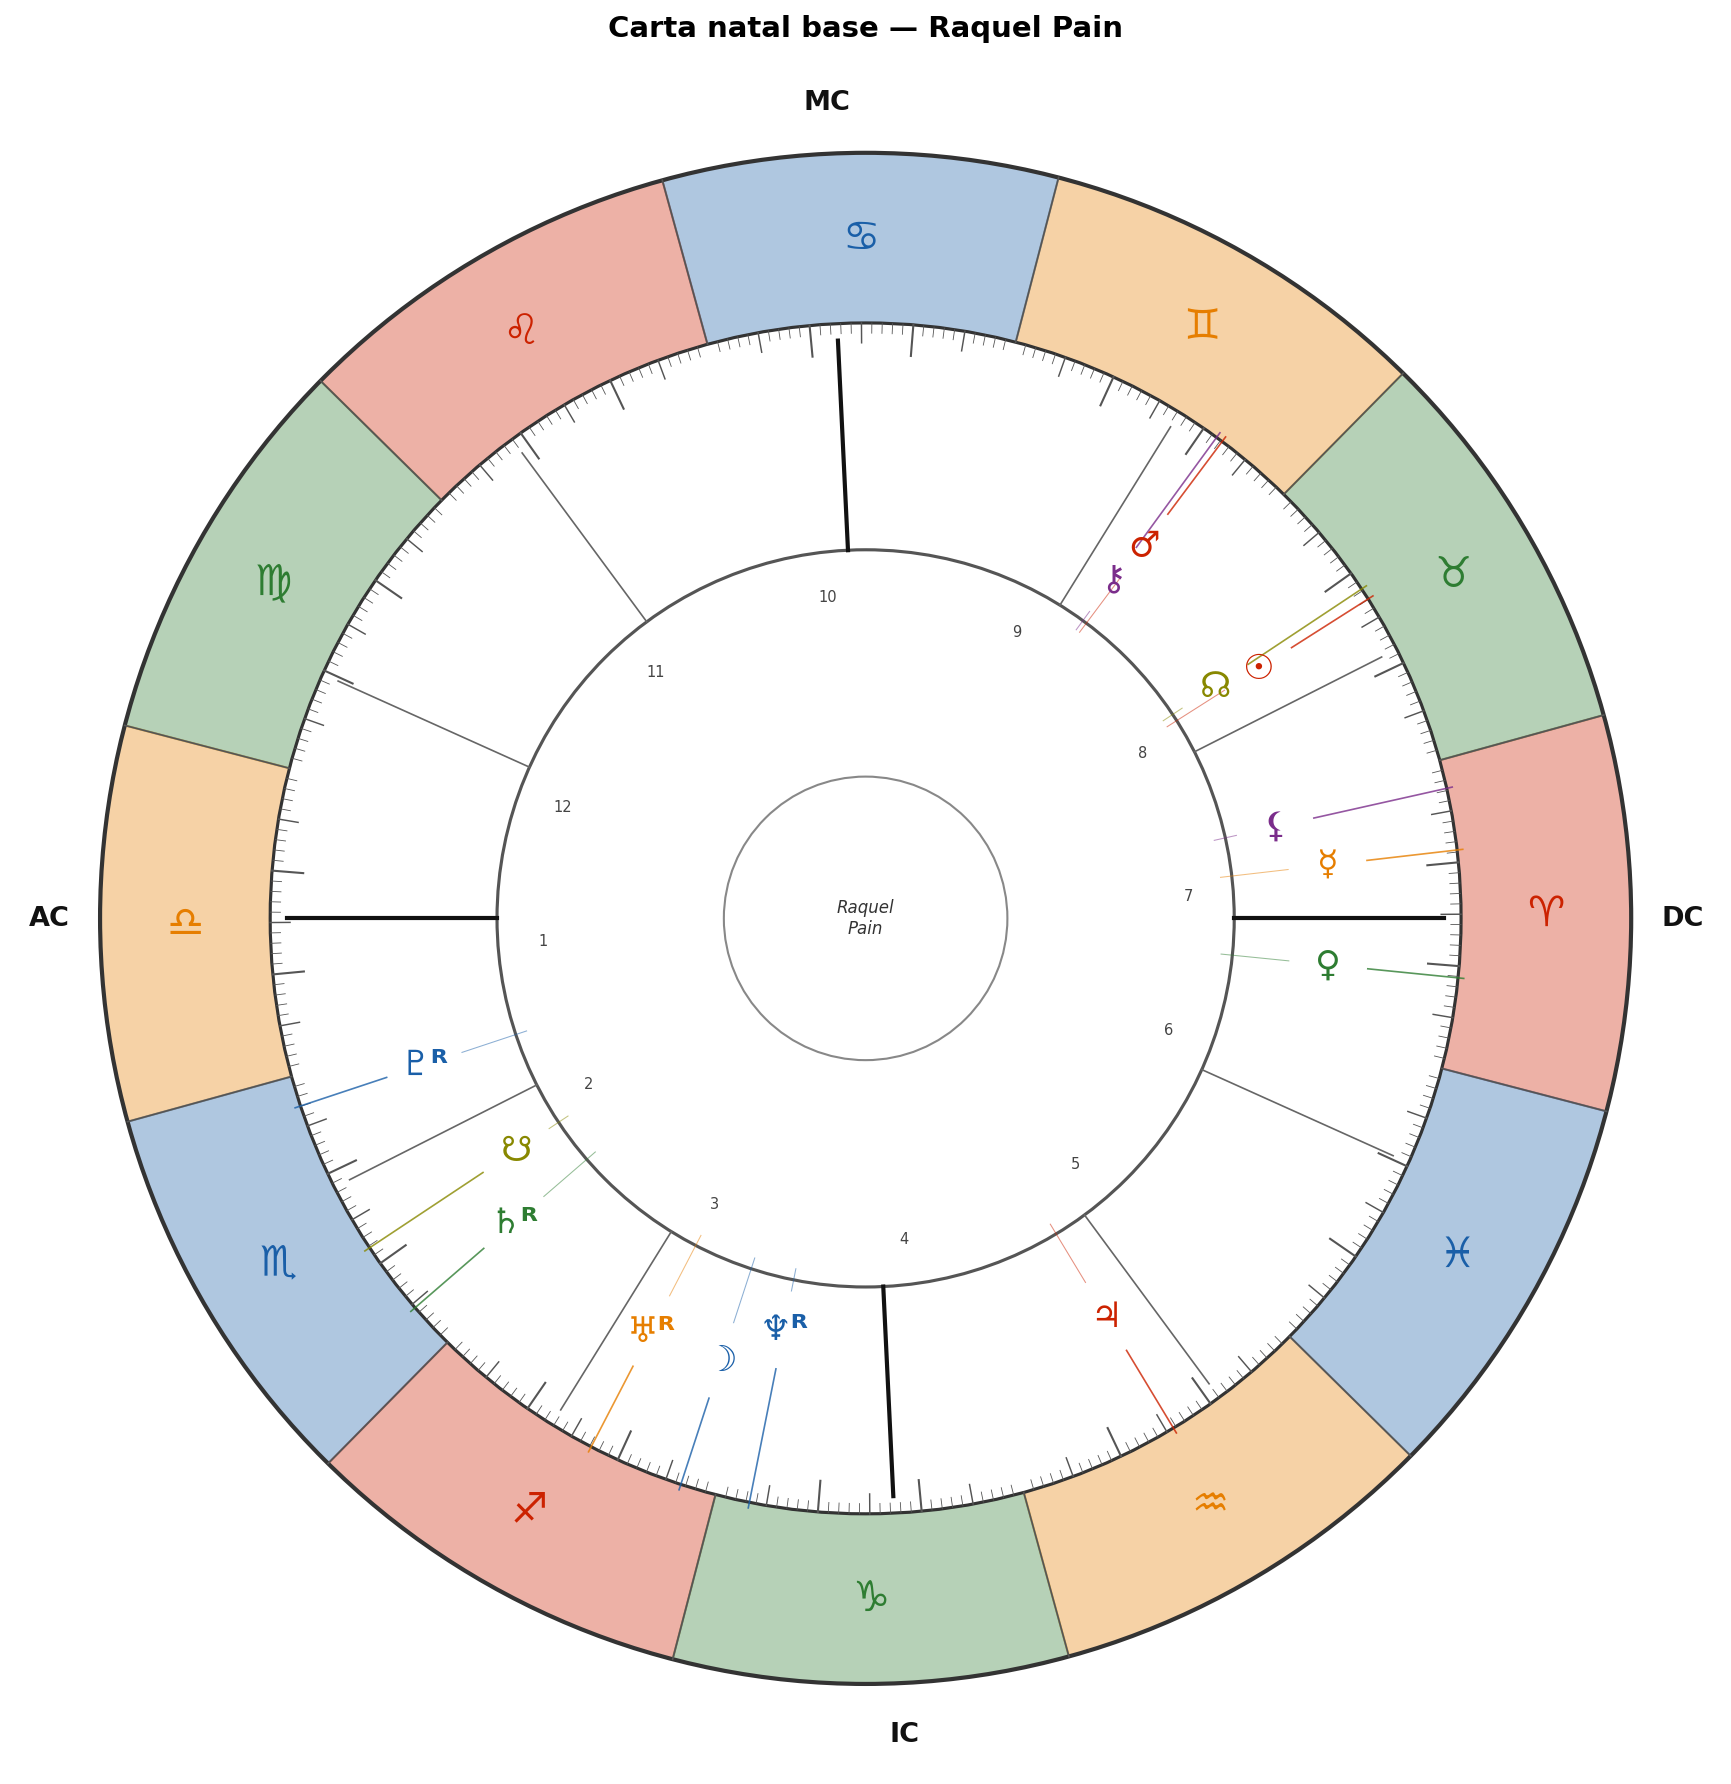
\includegraphics[width=0.8\textwidth]{Raquel_Pain_carta_base_rueda.png}
\end{center}

\vspace{0.8cm}

% ── POSICIONES PRINCIPALES ───────────────────────────────────────────────

\section{Posiciones principales}

\begin{center}

Sol en Tauro — Casa 8\\
Luna en Sagitario — Casa 3\\
Ascendente Libra\\
Medio Cielo en Cáncer

\end{center}

\vspace{0.5cm}

{\small\itshape
La lectura ampliada desarrolla el mapa completo de posiciones,
aspectos y configuraciones de la carta.
}

\vspace{0.8cm}
\Needspace{5\baselineskip}

% ── VISIÓN GENERAL ───────────────────────────────────────────────────────

\section{Visión general}

Tu carta muestra esta distribución de elementos: Fuego 7, Tierra 3, Aire 4.5, Agua 2. El elemento más presente es Fuego (iniciativa, impulso y necesidad de movimiento). Esto señala un registro que suele aparecer con facilidad en tu forma de funcionar. El elemento menos presente es Agua (sensibilidad, percepción emocional y conexión con el entorno). No significa ausencia, sino una cualidad que puede necesitar más atención consciente. Tu Medio Cielo en Cáncer orienta tu presencia pública hacia la cuidado, sensibilidad y atención a las necesidades humanas.

\vspace{0.8cm}
\Needspace{5\baselineskip}

% ── LOS TRES PILARES ────────────────────────────────────────────────────

\section{Los tres pilares}

\subsection{Sol en Tauro}

Con el Sol en Tauro, necesitas cierta estabilidad para sentirte bien con lo que construyes y con el ritmo de tu vida. Sueles valorar lo concreto, lo sencillo y aquello que puede sostenerse de forma real en el tiempo. Cuando algo te importa de verdad, normalmente puedes mantenerte con bastante constancia. Con el Sol en Casa 8, suele haber necesidad de profundidad, intensidad e implicación emocional. Las experiencias importantes normalmente tienden a afectarte de forma profunda, aunque no siempre lo muestres hacia fuera. Muchas veces necesitas sentir conexión real para implicarte de verdad con algo o con alguien.

\vspace{0.8cm}
\Needspace{5\baselineskip}

\subsection{Luna en Sagitario}

Con la Luna en Sagitario, necesitas espacio, movimiento y sensación de amplitud para sentirte bien emocionalmente. Sueles recuperar equilibrio cuando puedes cambiar de perspectiva, aprender algo nuevo o abrir horizontes. La sensación de crecimiento y dirección suele influir bastante en tu estado emocional. Con la Luna en Casa 3, las emociones suelen procesarse a través de la palabra, el pensamiento o la necesidad de compartir lo que ocurre. Hablar, escribir o entender mentalmente lo que sientes puede ayudarte bastante a encontrar claridad.

\vspace{0.8cm}
\Needspace{5\baselineskip}

\subsection{Ascendente Libra}

Con Ascendente en Libra, normalmente te muestras de forma amable, diplomática y orientada al vínculo con otras personas. Sueles percibir rápidamente cómo relacionarte con cada entorno o situación. Las demás personas suelen sentir facilidad y armonía en el primer contacto contigo.

\vspace{0.8cm}
\Needspace{5\baselineskip}

% ── CIERRE ───────────────────────────────────────────────────────────────

\section{Cierre}

Esta carta no busca definirte ni darte una identidad fija.

La astrología se utiliza aquí como lenguaje de observación:
una forma de mirar tendencias, ritmos y maneras de relacionarte con la vida.

La lectura ampliada desarrolla con más profundidad:
los vínculos,
la regulación emocional,
los patrones repetitivos,
la dirección de crecimiento,
las tensiones internas
y las configuraciones principales de la carta.

La lectura completa no busca darte más información.
Busca ayudarte a entender cómo sostener tu vida sin romperte por dentro.

\vspace{1cm}

\begin{center}

{\small\itshape\color{grisai}
Arquitectura Interna
}

\end{center}

\end{document}
